\pagebreak
\subsection{Symbole}
Die Vanille Symbole werden auf der Karte gesetzt in dem man, im Kartenmenü, per Doppelklick auf die gewünschte Position einen Punkt setzt. Standardmäßig kann mit den Cursor Pfeilen >> \begin{math} \uparrow,\downarrow \end{math} << die Symbole durchgeschaltet werden. Mit >>Shift<< wird die Farbe geändert. Eine Rotation der Pfeile ist leider nicht vorgesehen. \\
Die Vanille Kartenmarkierungen sollten nur im "Gruppen Channel" gesetzt werden.

\begin{longtable}{C{0.1\linewidth} m{0.85\linewidth}}
	\includegraphics[scale=0.8]{../img/advanced/kartenarbeit/hq}	& 	Hauptquartier / Stützpunkt \\
	\includegraphics[scale=0.8]{../img/advanced/kartenarbeit/punkt}	&	Punkt, grün Haus sauber, oder auch Wegpunkte \\
	\includegraphics[scale=0.8]{../img/advanced/kartenarbeit/pfeil}	&	Pfeil / Richtung \\
	\includegraphics[scale=0.8]{../img/advanced/kartenarbeit/start}	&	Startpunkt \\
	\includegraphics[scale=0.8]{../img/advanced/kartenarbeit/endpunkt}	&	Endpunkt \\
	\includegraphics[scale=0.8]{../img/advanced/kartenarbeit/treffpunkt}	&	Treffpunkt \\
	\includegraphics[scale=0.8]{../img/advanced/kartenarbeit/aufgabe}	&	Aufgabe / Ziel \\
	\includegraphics[scale=0.8]{../img/advanced/kartenarbeit/angriffsrichtung}	& 	Angriffsrichtung \\
	\includegraphics[scale=0.8]{../img/advanced/kartenarbeit/achtung}	&	Vorsicht / Warnung \\
	
\includegraphics[scale=0.8]{../img/advanced/kartenarbeit/frage_unbekannt}	& 	Unbekannt \\
	\includegraphics[scale=0.8]{../img/advanced/kartenarbeit/lz}	&	Landezone
\end{longtable}

\newpage
Kartenmarkierungen werden auf dem Tablet über ein Dropdownmenü aufgerufen. Über den Punkt Salute Reports und Route Planing werden die Unterpunkte aufgerufen. Bei Salute Reports kann man Einheiten melden, Art, Stärke und Richtung. Über das Route Planing kann man die restlichen Symbole einfügen.

\begin{longtable}{C{0.1\linewidth} m{0.85\linewidth}}
	\includegraphics[scale=0.8]{../img/advanced/kartenarbeit/unbekannt}	& 	Unbekannt \\
	\includegraphics[scale=0.8]{../img/advanced/kartenarbeit/recon}	& 	Recon / Späher \\
	
\includegraphics[scale=0.8]{../img/advanced/kartenarbeit/motorisierte_infanterie}	& 	motorisierte Infanterie \\
	
\includegraphics[scale=0.8]{../img/advanced/kartenarbeit/mechanisierte_infanterie}	& 	mechanisierteInfanterie\\
	\includegraphics[scale=0.8]{../img/advanced/kartenarbeit/panzer}	& 	Panzer \\
	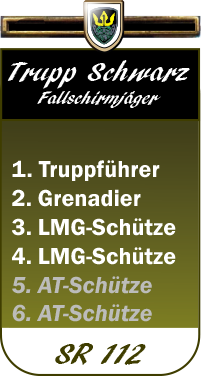
\includegraphics[scale=0.8]{../img/advanced/kartenarbeit/infanterie}	& 	Infanterie \\
	\includegraphics[scale=0.8]{../img/advanced/kartenarbeit/flugzeug}	& 	Flugzeug \\
	\includegraphics[scale=0.8]{../img/advanced/kartenarbeit/hubschrauber}	&	 Hubschrauber \\
	\includegraphics[scale=0.8]{../img/advanced/kartenarbeit/drohne}	& 	Drohne \\
\end{longtable}